\acf{top} is a new programming paradigm used to develop online collaborative applications. In a \acs{top} application, users - both people and other systems - work together to accomplish a common goal. Its central concept is called a Task, an abstraction that can be used for many different types of work. This abstraction, along with other TOP concepts, allows the user to focus on design decisions instead of technical details. TOP programs are declarative: they focus on \textit{what} work the user performs, rather than on \textit{how} to perform it.

\section{iTasks}\label{itasks}
iTasks is an \acs{edsl} that implements the \acs{top} paradigm. Its host language is the pure and lazy functional programming language \textit{Clean}. iTasks uses generic programming to automatically generate code for user-specified data types whilst also allowing for specialization. Given an iTask program, the system generates code for both the server and the client.

An iTask Task is a function that consumes a state and returns a \texttt{TaskValue} of type \texttt{a}, where \texttt{a} is the type of the task (represented by \texttt{Task a}). A \texttt{TaskValue} contains the current state of the value that a Task is processing. The possible states of a \texttt{TaskValue} are shown on Figure \ref{fig:task_value}. As we can see below, once a value stabilizes, it can not become unstable anymore.


\begin{figure}[H]
\begin{center}
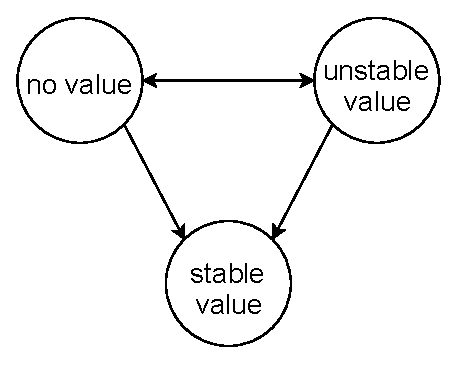
\includegraphics[scale=0.7]{thesis/img/task_value.eps}
\end{center}
\caption{Possible states of a \texttt{TaskValue}}
\label{fig:task_value}
\end{figure}

A Task can be of any type, as long as there is an instance of the \texttt{iTask} type class to it. This instance can be automatically derived or explicitly declared. Automatic derivation is available for any type as long as it is not abstract, extendable or the function type. Basic types have instances already declared in the iTasks library. Explicit declaration allows the user to define a custom instance of the \texttt{iTask} type class if the default derived instance is not suitable. In addition, it allows instances for extendable, abstract and the function types. 

\section{Interaction}\label{interaction}

The iTasks library provides basic tasks for interacting with the user. Listing \ref{l_top1} shows the three basic interactive tasks: \texttt{enterInformation}, \texttt{viewInformation} and \texttt{updateInformation}. They create user interface elements to enter, view and update information respectively. Notice that on all of the taks below, there is a constraint which requires that the type \texttt{m} of the returned \texttt{Task} must implement an instance of the \texttt{iTask} type class. 

\begin{lstlisting}[caption=iTasks basic interaction functions,captionpos=b,label=l_top1]
class toPrompt d where
    toPrompt :: !d -> UI

enterInformation :: !d ![EnterOption m] -> Task m | toPrompt d & iTask m
viewInformation :: !d ![ViewOption m] !m -> Task m | toPrompt d & iTask m
updateInformation :: !d ![UpdateOption m m] m -> Task m | toPrompt d & iTask m 
\end{lstlisting}


Listing \ref{l_top2} displays examples of how to use these tasks. We introduce a new \ac{adt}, called \texttt{Location} and automatically derive its instance of the \texttt{iTask} type class. Following, we introduce a new example location. Finally, we define tasks based on the basic tasks defined in Listing \ref{l_top1}. Here, keep in mind that the iTasks standard library implements an instance of the \texttt{toPromt} type class for the type \texttt{String}.  


\begin{lstlisting}[caption=Example of basic iTask interaction functions,captionpos=b,label=l_top2]
:: Location = { city :: String, state :: String }

derive class iTask Location

location :: Location
location = { city="Omaha", state="Nebraska"}

enterLocation :: Task Location
enterLocation = enterInformation "Enter the location" []

viewLocation :: Task Location
viewLocation = viewInformation "View the location" [] location

updateLocation :: Task Location
updateLocation = updateInformation "Update the location" [] location
\end{lstlisting}

Figure \ref{fig:itasks_display} displays the user interfaces generated for the basic tasks \texttt{enterInformation} (Figure \ref{fig:enter_info}), \texttt{viewInformation} (Figure \ref{fig:view_info}) and \texttt{updateInformation} (Figure \ref{fig:upd_info}).

\begin{figure}[H]
\begin{subfigure}{0.33\textwidth}
\includegraphics[scale=0.7]{thesis/img/enter_location.png}
\caption{Enter Information}
\label{fig:enter_info}
\end{subfigure}
\begin{subfigure}{0.33\textwidth}
\includegraphics[scale=0.55]{thesis/img/view_location.png}
\caption{View Information}
\label{fig:view_info}
\end{subfigure}
\begin{subfigure}{0.33\textwidth}
\includegraphics[scale=0.7]{thesis/img/update_location.png}
\caption{Update Information}
\label{fig:upd_info}
\end{subfigure}
\caption{The visual representation of the basic iTask interaction functions}
\label{fig:itasks_display}
\end{figure}


\section{Combinators}\label{combinators}

Although the basic tasks introduced in Section \ref{interaction} allow the user to exchange information with the iTasks application, they are quite limited. In order to allow the user to express more complex behavior, task combinators were introduced. Combinators are functions (usually infix operators) that determine how its argument tasks will be combined into a new task. There are only two fundamental combinators, sequence and parallel. All the other combinators in the \texttt{iTask} library are defined based on these fundamental combinators.

\subsection{Sequential Combinator}
\begin{lstlisting}[caption=Sequential Combinators,label=seq_comb,captionpos=b]
(>>*) infixl 1 :: !(Task a) ![TaskCont a (Task b)] -> Task b | iTask a & iTask b

:: TaskCont a b                               
	= OnValue ((TaskValue a) -> Maybe b)         
	| OnAction Action ((TaskValue a) -> Maybe b) 
	| E.e: OnException (e -> b) & iTask e        
	| OnAllExceptions (String -> b)    
\end{lstlisting}

\subsection{Parallel Combinators}

\begin{lstlisting}[caption=Parallel Combinators,label=par_comb,captionpos=b]
(-||-) infixr 3 :: !(Task a) !(Task a) -> Task a | iTask a
(-&&-) infixr 4 :: !(Task a) !(Task b) -> Task (a,b) | iTask a & iTask b
\end{lstlisting}


\section{Shared Data Sources}
